%%%%%%%%%%%%%%%%%%%%%%%%%%%%%%%%%%%%%%%%%%%%%%%%%%%%%%%%%%%%%%%%%
%% TITLE PAGE.
%%%%%%%%%%%%%%%%%%%%%%%%%%%%%%%%%%%%%%%%%%%%%%%%%%%%%%%%%%%%%%%%%

% No headers or footers on the title page.
\thispagestyle{empty}

\begin{titlepage}
\centering
\setstretch{1.0}
\null
\vspace*{0.25in}
\UseLMSSBoldFont\huge
Insert Thesis Title Here
\\[0.25em]
Use Multiple Lines If Necessary
\\[0.4in]
\normalfont\large
Thesis by
\\[0.25em]
\UseLMSSBoldFont\Large
Insert Author Name Here
\\[0.4in]
\normalfont\normalsize
In Partial Fulfillment of the Requirements
\\[0.5em]
for the Degree of
\\[0.5em]
Doctor of Philosophy
\vfill
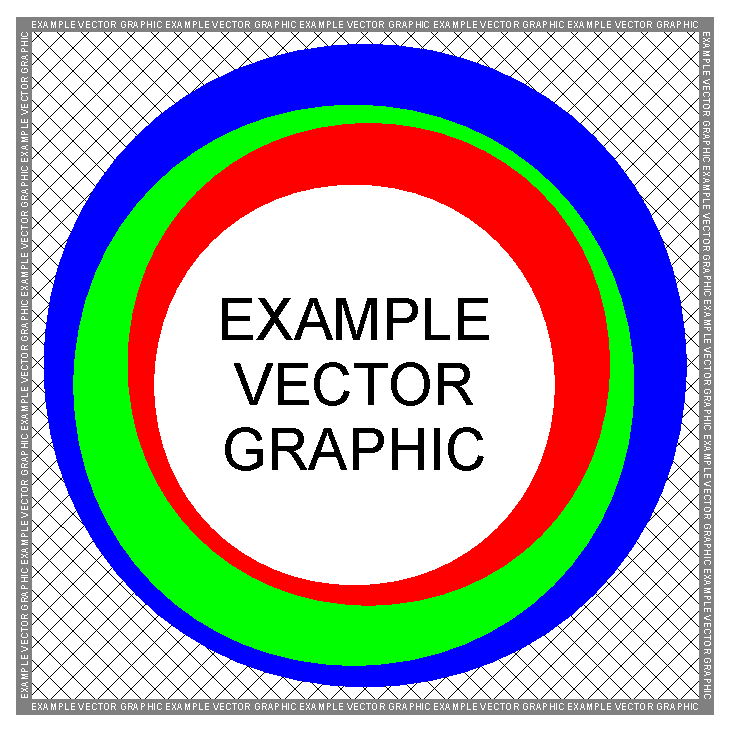
\includegraphics[height=1.8in]
{Figure-SchoolLogo}
\\[0.5em]
University Institute of College
\\[0.5em]
Springfield, New York, USA
\\[1.5em]
2014
\\[0.5em]
(Defended January 7, 2014)
\par
\end{titlepage}

%%%%%%%%%%%%%%%%%%%%%%%%%%%%%%%%%%%%%%%%%%%%%%%%%%%%%%%%%%%%%%%%%
%% COPYRIGHT PAGE.
%%%%%%%%%%%%%%%%%%%%%%%%%%%%%%%%%%%%%%%%%%%%%%%%%%%%%%%%%%%%%%%%%

\pagestyle{plain}
\setcounter{page}{2}

{\centering
\null
\vfill
\raisebox{0.15em}{\scriptsize\sffamily\textcopyright}~2014
\\
Insert Author Name Here
\\
All Rights Reserved
\par}

\clearpage

%%%%%%%%%%%%%%%%%%%%%%%%%%%%%%%%%%%%%%%%%%%%%%%%%%%%%%%%%%%%%%%%%
%% DEDICATION PAGE.
%%%%%%%%%%%%%%%%%%%%%%%%%%%%%%%%%%%%%%%%%%%%%%%%%%%%%%%%%%%%%%%%%

{\centering
\null
\vspace*{1in}
\textit{Insert dedication here}
\par}

\clearpage

%%%%%%%%%%%%%%%%%%%%%%%%%%%%%%%%%%%%%%%%%%%%%%%%%%%%%%%%%%%%%%%%%
%% ACKNOWLEDGMENTS.
%%%%%%%%%%%%%%%%%%%%%%%%%%%%%%%%%%%%%%%%%%%%%%%%%%%%%%%%%%%%%%%%%

\chapter*{Acknowledgments}
\addcontentsline{toc}{chapter}{Acknowledgments}

Insert thesis acknowledgments here.
Thesis acknowledgments typically include research advisers and mentors, thesis committee members, collaborators, and funding sources.

\lipsum[1-2]

\clearpage

%%%%%%%%%%%%%%%%%%%%%%%%%%%%%%%%%%%%%%%%%%%%%%%%%%%%%%%%%%%%%%%%%
%% ABSTRACT.
%%%%%%%%%%%%%%%%%%%%%%%%%%%%%%%%%%%%%%%%%%%%%%%%%%%%%%%%%%%%%%%%%

\chapter*{Abstract}
\addcontentsline{toc}{chapter}{Abstract}

Insert thesis abstract here.
The thesis abstract provides a concise description of the main contributions in the thesis.
Abstracting and indexing services usually include the thesis abstract in the catalog presented to users.
A well-written abstract could improve the chances of your work being discovered and cited by others in the research community.
The abstract should be self-contained (avoid citations and cross references) and should contain only plain text (avoid complicated mathematical expressions).

\lipsum[1-6]

\clearpage

%%%%%%%%%%%%%%%%%%%%%%%%%%%%%%%%%%%%%%%%%%%%%%%%%%%%%%%%%%%%%%%%%
%% TABLE OF CONTENTS (TOC), LISTS OF FIGURES/TABLES/ETC.
%%%%%%%%%%%%%%%%%%%%%%%%%%%%%%%%%%%%%%%%%%%%%%%%%%%%%%%%%%%%%%%%%

\tableofcontents

\listoffigures

\listoftables

\clearpage
